


%% bare_jrnl.tex
%% V1.4a
%% 2014/09/17
%% by Michael Shell
%% see http://www.michaelshell.org/
%% for current contact information.
%%
% *** Do not adjust lengths that control margins, column widths, etc. ***
% *** Do not use packages that alter fonts (such as pslatex).         ***
% There should be no need to do such things with IEEEtran.cls V1.6 and later.
% (Unless specifically asked to do so by the journal or conference you plan
% to submit to, of course. )

\documentclass[journal]{IEEEtran}

%\usepackage{cite}
% Better looking tables
%\usepackage{array}

% correct bad hyphenation here
\hyphenation{op-tical net-works semi-conduc-tor}

% Some stuff mox needs:
\usepackage{graphicx}
\graphicspath{{../material/paper/}}

\usepackage{hyperref}
%\definecolor{darkblue}{rgb}{0,0,.5}
%\hypersetup{pdftex=true, colorlinks=true, breaklinks=true, linkcolor=darkblue, menucolor=darkblue, pagecolor=darkblue, urlcolor=darkblue}
\hypersetup{pdftex=true, colorlinks=false, breaklinks=true}

%\usepackage[usenames,dvipsnames]{xcolor}
\usepackage{tkz-kiviat,numprint,fullpage}
\usetikzlibrary{arrows}

\usepackage{xcolor}
\usepackage{minted}

\usepackage{lipsum}
\usepackage{xspace}
\newcommand{\twi}{I\textsuperscript{2}C\xspace}
\newcommand{\mosi}{\texttt{MOSI}\xspace}
\newcommand{\miso}{\texttt{MISO}\xspace}
\newcommand{\clock}{\texttt{CLOCK}\xspace}
\renewcommand{\ss}{\texttt{\textoverline{SS}}\xspace}

\newcommand{\sda}{\texttt{SDA}\xspace}
\newcommand{\scl}{\texttt{SCL}\xspace}
\newcommand{\startcondition}{\texttt{START} condition\xspace}
\newcommand{\stopcondition}{\texttt{STOP} condition\xspace}
\newcommand{\clockstretching}{\texttt{CLOCK STRETCHING}\xspace}
\newcommand{\ack}{\texttt{ACK}\xspace}
\newcommand{\nak}{\texttt{NACK}\xspace}

\makeatletter
\newcommand*{\textoverline}[1]{$\overline{\hbox{#1}}\m@th$}
\makeatother

\begin{document}
 %\setlength{\parindent}{0mm}
\title{Industry Standard Control Interfaces\\for inter IC communication}
%
%
% author names and IEEE memberships
% note positions of commas and nonbreaking spaces ( ~ ) LaTeX will not break
% a structure at a ~ so this keeps an author's name from being broken across
% two lines.
% use \thanks{} to gain access to the first footnote area
% a separate \thanks must be used for each paragraph as LaTeX2e's \thanks
% was not built to handle multiple paragraphs
%

%\author{Moritz~N\"oltner%
%	\IEEEcompsocitemizethanks{\IEEEcompsocthanksitem M. N\"oltner is enrolled at the University of Heidelberg and is currently pursuing a B.S. degree in applied informatics.\protect\\
%	E-mail: sh386@ix.urz.uni-heidelberg.de}%
%\thanks{Manuscript received January 6, 2015; revised January 12, 2015.}}%

\author{Moritz~N\"oltner\\%
		University of Heidelberg, ZITI}
%	\IEEEcompsocitemizethanks{\IEEEcompsocthanksitem M. N\"oltner is enrolled at the University of Heidelberg and is currently pursuing a B.S. degree in applied informatics.\protect\\
%	E-mail: sh386@ix.urz.uni-heidelberg.de}%
%\thanks{Manuscript received January 6, 2015; revised January 12, 2015.}}%

% The paper headers
\markboth{Advanced Seminar "`Computer Engineering"', UNIVERSITY OF HEIDELBERG WT14/15}%
{Shell \MakeLowercase{\textit{et al.}}: Industry Standard Control Interfaces\\for inter IC communication}

% use for special paper notices
%\IEEEspecialpapernotice{(Invited Paper)}

\maketitle

% As a general rule, do not put math, special symbols or citations
% in the abstract or keywords.
\begin{abstract}
This paper gives a short overview of the \twi (Inter-Integrated Circuit) and SPI (Serial Peripheral Interface) bus systems and showcases a record of a typical \twi transaction.
\end{abstract}

% Note that keywords are not normally used for peerreview papers.
\begin{IEEEkeywords}
System buses, SPI, \twi, Two Wire Interface.
\end{IEEEkeywords}

% For peer review papers, you can put extra information on the cover
% page as needed:
% \ifCLASSOPTIONpeerreview
% \begin{center} \bfseries EDICS Category: 3-BBND \end{center}
% \fi
%
% For peerreview papers, this IEEEtran command inserts a page break and
% creates the second title. It will be ignored for other modes.
\IEEEpeerreviewmaketitle



\section{Introduction}
% The very first letter is a 2 line initial drop letter followed
% by the rest of the first word in caps.
% 
% form to use if the first word consists of a single letter:
% \IEEEPARstart{A}{demo} file is ....
% 
% form to use if you need the single drop letter followed by
% normal text (unknown if ever used by IEEE):
% \IEEEPARstart{A}{}demo file is ....
% 
% Some journals put the first two words in caps:
% \IEEEPARstart{T}{his demo} file is ....
% 
\IEEEPARstart{I}{n} computer systems, different parts of the circuit will need to exchange data and configuration information. To facilitate this, a vast number of data link systems have been used which are distinguishable in terms of complexity, data throughput and whether they are point-to-point connections or bus systems.
Some notable examples of data link systems in roughly descending order of complexity are:
\renewcommand{\labelitemi}{$-$}
%\renewcommand{\labelitemi}{$\circ$}
\begin{itemize}
		\item HyperTransport
		\item PATA, SATA
		\item PCI, PCI-Express
		\item AGP
		\item ISA
		\item CAN
		\item UART, USART
		\item SPI
		\item \twi, SMBus
		\item UNI/O
		\item 1-Wire
\end{itemize}
\IEEEPARstart{}{}Along with USART (Universal [Asynchronous] Receiver Transmitter), SPI (Serial Peripheral Interface) and \twi (Inter-Integrated Circuit) are probably the most commonly used data links for low speed, low complexity interfacing of integrated circuits (ICs). SPI and \twi are special in that they are bus systems, which means that a possibly large number of ICs can share the same signal lines for communication.


\section{Serial Peripheral Interface}
The Serial Peripheral Interface was introduced by Motorola for the 6800 series of processors, though Texas Instruments introduced a similar system, Microwire\cite{microwire}. It allows to communicate to external components by using a simple, yet versatile 4-wire bus system with dedicated chip select, clock and data lines. By now, SPI has become a widely accepted de-facto standard with microcontrollers, digital signal processors, FLASH memories, ADCs and DACs and many sensors offering an SPI interface.

\subsection{Technical Description}
The SPI connects one master and any number of slaves. The master is the device that controls the transactions and provides the clock signal. There are three signal lines common to all participants. These are \clock, \mosi and \miso and one line specific to each slave, \ss.
\begin{description}
	\item[\mosi] Master~Out, Slave~In\\This line carries the serial data, the master sends for the slave to receive with the most significant bit first.
	\item[\miso] Master~in, Slave~Out\\ This line carries the slave's serial data to the master, again with the most significant bit first.
	\item[\clock] The synchronisation clock the master sends to synchronise with a slave. During each clock cycle, one bit of information is sent by master and slave each.
	\item[\ss] Slave~Select\\ The master asserts this line for a slave prior to starting a transaction with it by tieing it to a low level. For all other slaves, this line has to be at a logical high level, therefore deasserted. A slave, whose slave select is active will configure it's \mosi pin as input and \miso pin as output. All other slaves must disconnect themselves from the bus. This means, these slaves must not effect any changes on the bus lines and not be affected by the ongoing transaction.
\end{description}
The basic part of an SPI device is a shift register with an additional parallel access tap to write and read data. The \mosi line is connected to the shift out of the masters shift register and to the shift in of the selected slaves shift register, and vice versa for the \miso line. The \ss will determine which slaves connects it's shift register to the bus. \clock controls the shifting. Depending on the settings for clock polarity and clock phase, 4 modes are possible, which differ in when data is applied on the bus lines, and when it is sampled according to the clock cycle.  See figure~\ref{simple_spi_con} for details on the connections and figure~\ref{spi_cpol_cpha} for details on the clock signal.

\begin{figure}[!t]
\centering
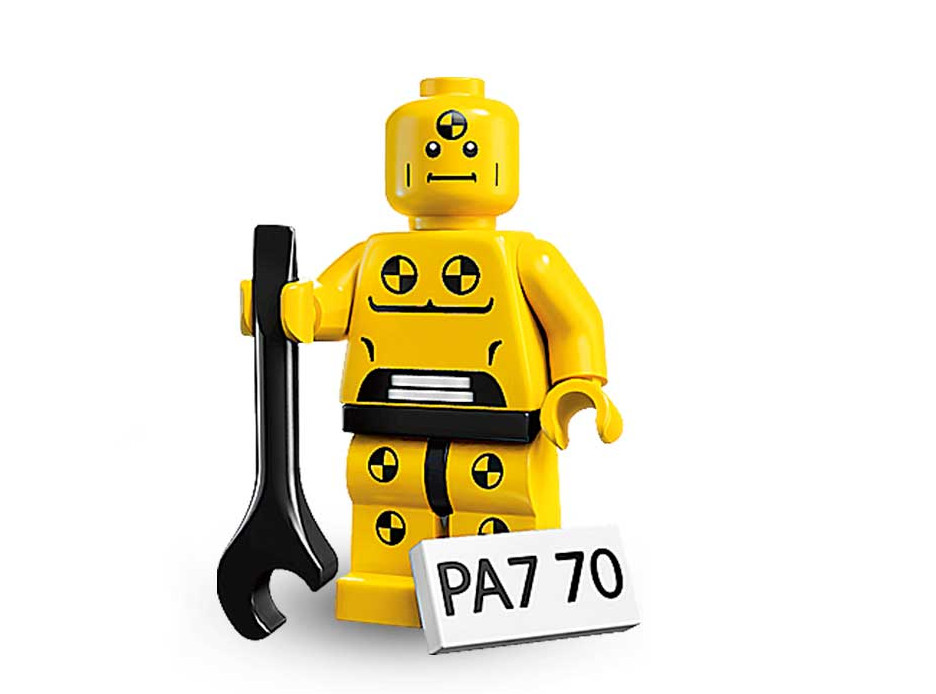
\includegraphics[width=3in]{dummy}
\caption{A simple connection between a master and one slave.\cite{spi_blockguide}}
\label{simple_spi_con}
\end{figure}

\begin{figure}[!t]
\centering
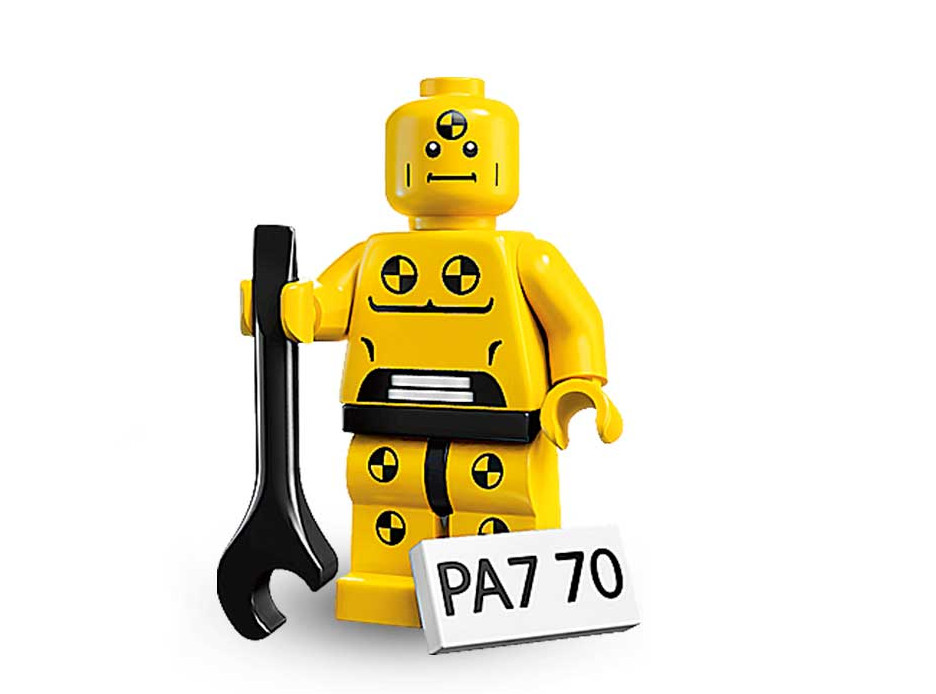
\includegraphics[width=3in]{dummy}
\caption{An example timing diagram showcasing clock phase and polarity.\cite{spi_c68hcp11a1vp}}
\label{spi_cpol_cpha}
\end{figure}

\subsection{Alternative Bus Topologies}
There are a number of possible alternations of the SPI connection:
\begin{description}
	\item [Star] All \mosi pins are tied together, all \clock pins are tied together and all \miso pins are tied together. The master controls the \ss line of each slave. This is the most typical topology.
	\item [Serial] A master is connected to a number of slaves which are daisy chained. All \ss pins can be tied together, or all the slaves \ss pins can be set to a low level.
\end{description}

\paragraph*{Star topology}
To address a slave and start a transaction, the master only has to pull that slave's \ss line low and start sending. After the frame is transmitted, master and slaves have exchanged the contents of their shift registers.
\paragraph*{Serial topology}
The master's \mosi pin is connected to the first slaves \mosi pin, the first slaves \miso pin is connected to the second slaves \mosi pin, whose \miso pin is connected to the third's \mosi pin and so on up to the last slave, whose \miso pin is connected to the master's \miso pin. The data sent over the bus will have to contain some address information and slaves which are not addressed by a data packet will have to pass it on through their \miso pin in the next frame. So, to address the n-th slave, the master will have to send a data packet for the n-th slave, and then n-1 more packets. During the transmission time of the n-1 packets, the data is passed on to the n-th slave. Then, to receive the response from the n-th slave, the master will have to continue sending until the response is passed through the remaining slaves. E.g. if there are a total of N slaves, the master will have to send N-n more packets.

Despite the obvious drawbacks, this topology provides two distinctive advantages over star topology:
% TODO: Quellen für den Multi-Master-Mode finden
\begin{enumerate}
	\item The master does not need to control all the possibly quite many \ss lines individually, therefore saving pins in i/o-pin restrained environments.
	\item If there are only two devices whose \ss pins are tied together, a multi-master communication becomes possible, because a master, whose \ss pin is pulled low, must switch to slave mode if supported.
\end{enumerate}


\section{Inter-Integrated Circuit}
The Inter-Integrated Circuit bus  is a simple ``snap-in" architecture developed by Philips, though some other companies use the name TWI for Two Wire Interface to avoid trademark conflicts pertaining to \twi \cite{twi1}\cite{twi2}. Devices can be added to or removed from the bus without the need to change anything else. The bus consists of just two wires and a pair of external pull-up resistors. The bus is designed for multi-master operation with collision detection being an integral part of the protocol. As with SPI, there are numerous devices of all kinds offering an \twi interface. On top of this, a number of other bus systems are compatible with devices prepared to operate in either system. Such bus systems include the System Management Bus (SMBus)\cite{pmbus} found in modern personal computers, Power Management Bus (PMbus)\cite{pmbus} and CBUS as stated in the \twi standard \cite{i2c_standard}. Figure~\ref{i2c_complete_connection} shows a (complex) setup of an \twi system. For a simpler setup, consider only the rightmost  part of the figure with the two F/S-mode devices, \sda and \scl lines, their pull-ups and $V_{DD2}$.

\subsection{Technical Description}
The \twi bus connects a number of devices, of which any can become master to begin a transaction. Because \twi is a half-duplex bus, meaning only one device can send data at a time, there are not only the roles of master, which will iniate a transaction, and slave, which has to respond to it, but also transmitter and receiver. A transmitter is the device sending data, a receiver receives it. All four combinations of master/slave and transmitter/receiver are possible. The two signal lines are called \sda and \scl. Each device should have an open-drain connection to those lines, as these, together with their pull-up resistors perform a wired-AND. The function of those lines is as follows:
\begin{description}
	\item[\scl] Serial Clock Line\\ The master applies it's clock to this line to synchronise with a slave. The slave can pull this line low to stretch the clock.
	\item[\sda] Serial Data Line\\ This line carries the data between master and slave and is used for handshaking.
\end{description}

\begin{figure*}[!t]
\centering
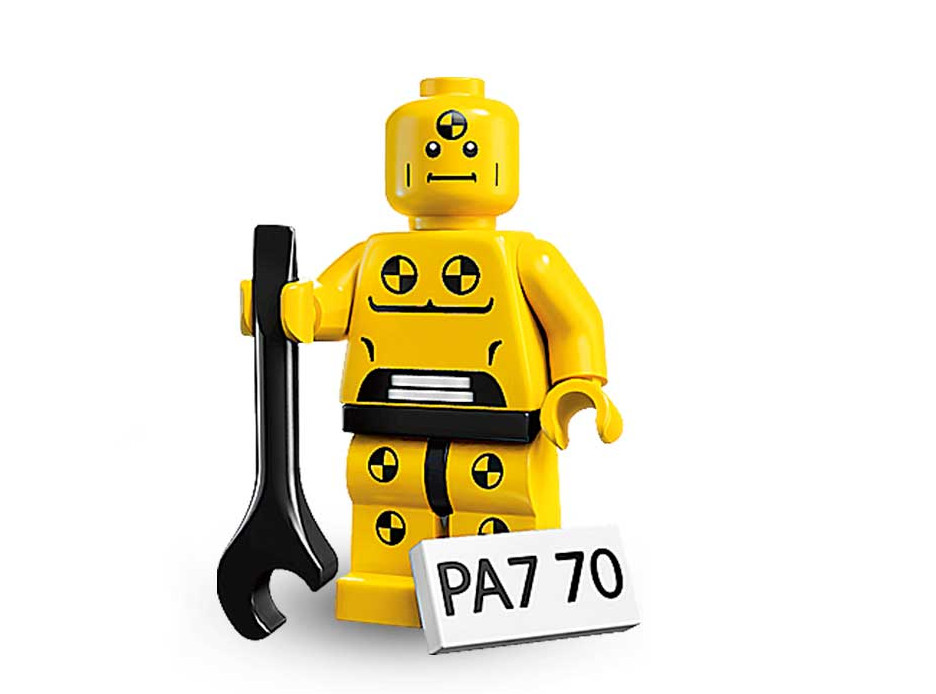
\includegraphics[width=0.95\linewidth]{dummy}
\caption{An example of an \twi read access.}
\label{i2c_transfer_complete}
\end{figure*}

\begin{figure*}[!t]
\centering
%\includegraphics[width=0.95\linewidth]{i2c_complete_connection_cropped}
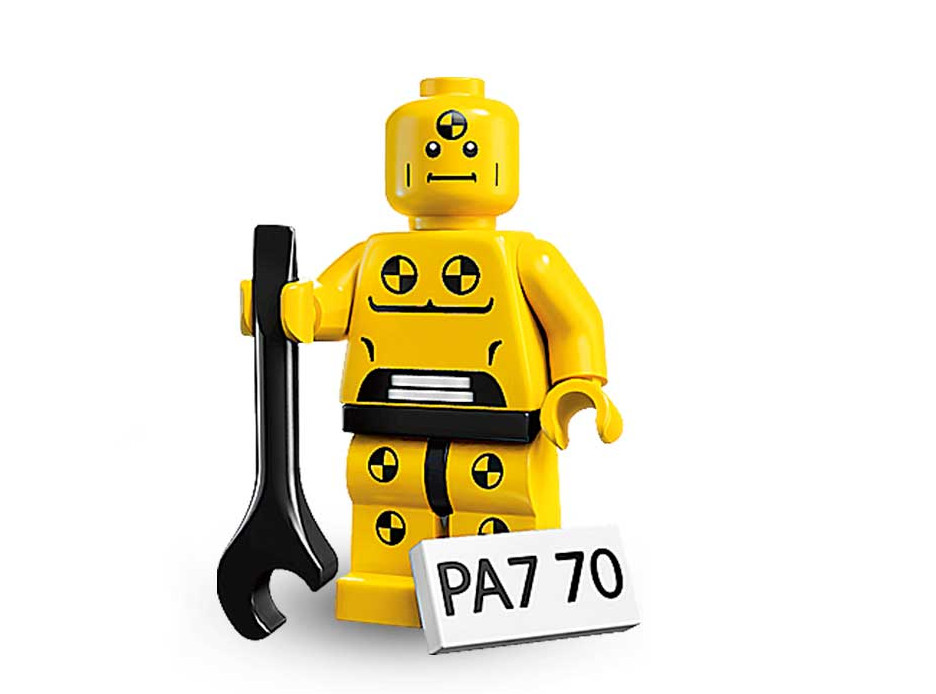
\includegraphics[width=0.95\linewidth]{dummy}
\caption{Mixing High-Speed and Full-Speed/Standard-Speed \twi devices.\cite{i2c_standard_v2.1}}
\label{i2c_complete_connection}
\end{figure*}

A transaction involves a device becoming master, addressing a slave, setting the read/write bit, receiving or sending some data and ending the transaction.
A device receiving data may use so called \clockstretching to slow down the transmitter.

\paragraph*{Becoming master of the bus}
In order to become master, the bus has to be free, then a device can issue a \startcondition to the bus. This means creating a negative-going edge on the bus.

\paragraph*{Sending an address or data}
During a transaction, the transmitter will put it's data onto the bus during the low part of the clock cycle, the receiver will latch this data during the high phase of the clock cycle. After eight bits, the transmitter will leave the \sda line floating and the receiver has to pull it low to acknowledge the reception. If there was an acknowledge, the transmitter will sent the next byte of data, if the receiver fails to pull the data line low, this means there was a not-acknowledge (\nak) and the master will issue either a \stopcondition, meaning a positive-going edge, become a slave again and free up the bus or issue a repeated \startcondition and start another transaction.
See figure~\ref{i2c_transfer_complete} for an example.

\paragraph*{\clockstretching}
If a slave cannot handle the transmission speed, it may slow down the transmission by prolonging the low phase of the \scl line.
The master will notice that the clock line did not rise to a high level when it turned of it's transistor pulling the line low, and will wait until the receiver releases the line before starting the next clock cycle and latching the next bit of data as receiver, or applying the next bit of data upon the bus as transmitter. Therefore \clockstretching enables devices of different speed grades to communicate with each other at the highest speed supported by both devices, but also allows a receiver which is ``distracted'', e.g. because it is serving an interrupt for a short time, to suspend a transaction. However, if a receiver is not able to accept new data, because a buffer is full, or some time-consuming calculations have to be done, it should \nak the reception of a byte of data, to tell the transmitter to abort the transaction and free the bus.


\subsection{Collision Detection and bus arbitration}
Collision detection and arbitration is implemented using the wired-AND functionality of the bus. Devices operating as masters have to probe the \sda line while transmitting. If two devices try to become master of the bus, both will issue a start condition and then begin to drive the clock line and send the address of the slave they want to access followed by the read/write bit and possibly their own data in case of a write. While both masters send exactly the same bit sequence, both will be masters. However, if one master sends a ``1'' while the other sends a ``0'', the master sending the ``1'' will recognise that the data line is also driven by another master (because the data line is at a logic low due to the wired-AND) therefore lose the arbitration and silently become a slave for the rest of the transaction. Data integrity is ensured because the losing master became a slave before any race condition could occur.

\subsection{10-bit Addressing}
The original specification of \twi had 7 bits of address information and one bit specifying whether a read or write was to be performed. This was to be the first byte sent. With 16 addresses reserved for various reasons listed in figure~\ref{i2c_addresses}, this left a total of 112 distinguishable addresses. When \twi gained popular acceptance, a need for further addresses arose, and thus 10-bit addressing was introduced. While there will seldom be that many devices on one bus, address clashes can occur with just a few devices, because the addresses are hardcoded, even though some devices allow programing one or two bits by tying pins to ground or $V_{cc}$. Figure~\ref{i2c_10_bit_addressing} shows the pattern of 10-bit addressing.

To retain downward compatibility, 10-bit addressing uses a concatenation of 11110 + the first 2 bits of the 10-bit address + the R/\textoverline{W}-bit as the first transmitted byte, with the remaining 8 bits of the address being the second transmitted byte. 11110XX were reserved addresses, to which no device was allowed to respond. A device which utilises 10-bit addressing will acknowledge the reception of the first byte, if the first two bits of the match. If later on, the rest of the address matches, too, it will acknowledge the second byte as well and be addressed, else it will not acknowledge the second byte and retreat from the transaction.

\begin{figure}[!t]
\centering
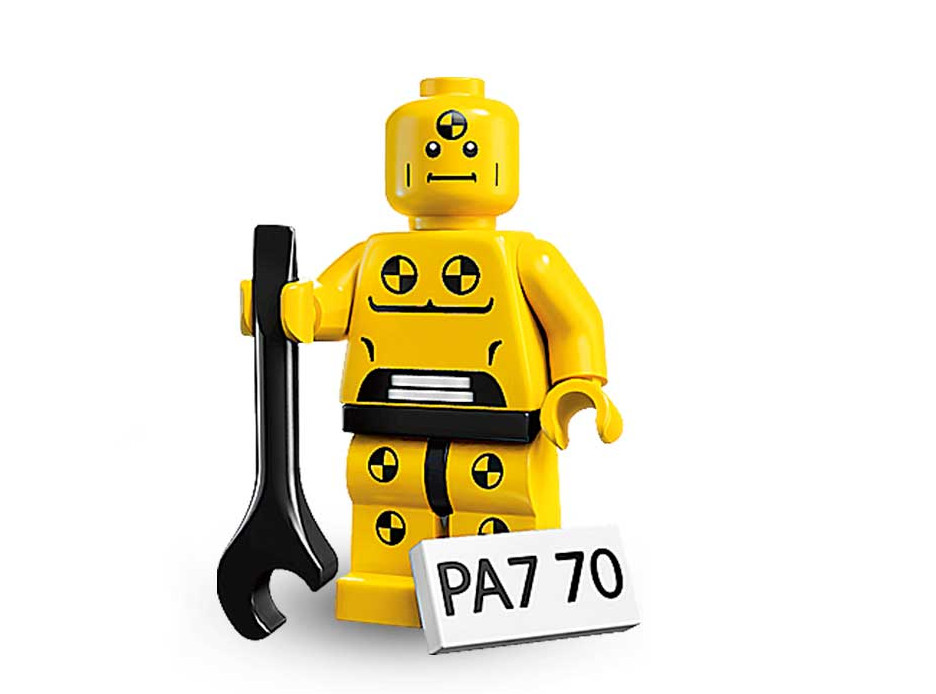
\includegraphics[width=3in]{dummy}
\caption{Structure of a transaction with 10-bit addressing. Adapted~from~\cite{i2c_standard}}
\label{i2c_10_bit_addressing}
\end{figure}

\begin{table}[!t]
\renewcommand{\arraystretch}{1.3}
\caption{Reserved \twi Addresses.\cite{i2c_standard}}
\label{i2c_addresses}
\centering
\begin{tabular}{lll}
\hline
Address & R/\textoverline{W}-Bit & Description\\
\hline
0000 000 & 0 & general call address\\
0000 000 & 1 & START byte\\
0000 001 & X & CBUS address\\
0000 010 & X & reserved for different bus format\\
0000 011 & X & reserved for future purposes\\
0000 1XX & X & Hs-mode master code\\
1111 1XX & 1 & device ID\\
1111 0XX & X & 10-bit slave addressing\\
\hline
\end{tabular}
\end{table}

\subsection{Higher Communication Speeds}
In Standard-Mode, communication at up to 100 kbit/s is possible, Fast-Mode provides 400 kbit/s and Fast-Mode Plus allows up to 1 Mbit/s. To achieve this increase in speed, some timing restraints were loosened and for the Fast-Mode Plus, the drive strength of the devices was increases up to tenfold, but the protocol remained unchanged except for the increased speed.

The next speed step is at 3.4 Mbit/s and is called High-Speed Mode. This mode is not backwards compatible, the changes include:
\begin{itemize}
	\item A pull-up current source for the signal lines in each master to reduce the signal rise time.
	\item Spike suppression and schmitt triggers have been added to the inputs.
	\item Clock stretching may only occur after the \ack bit, during a transfer, the slaves may not interfere with the clock signal.
	\item To initiate a High-Speed Mode transaction, the master will first have to transmit a master code while operating in Fast-Mode. This code, which is 0000 1XX, will tell the other devices that the master would like to start a High-Speed-Mode transfer.
	\item No bus arbitration is possible while in High-Speed-Mode. Arbitration happens exclusivly during the Fast-Mode-transmission of the master code, whose last three digits can be chosen by the system designer. This way, up to 7  high-speed masters can operate on the bus and complete arbitration within the transmission of the first byte.
\end{itemize}

To increase the speed even further, there is an Ultra-Fast-Mode with up to 5 Mbit/s. Although the bus protocol remains the same as with the other modes, only unidirectional communication is supported, and Ultra-Fast-Mode devices use push-pull output stages, making them incompatible with other \twi-standards.

\section{Recording \twi}
\begin{figure}[!t]
\centering
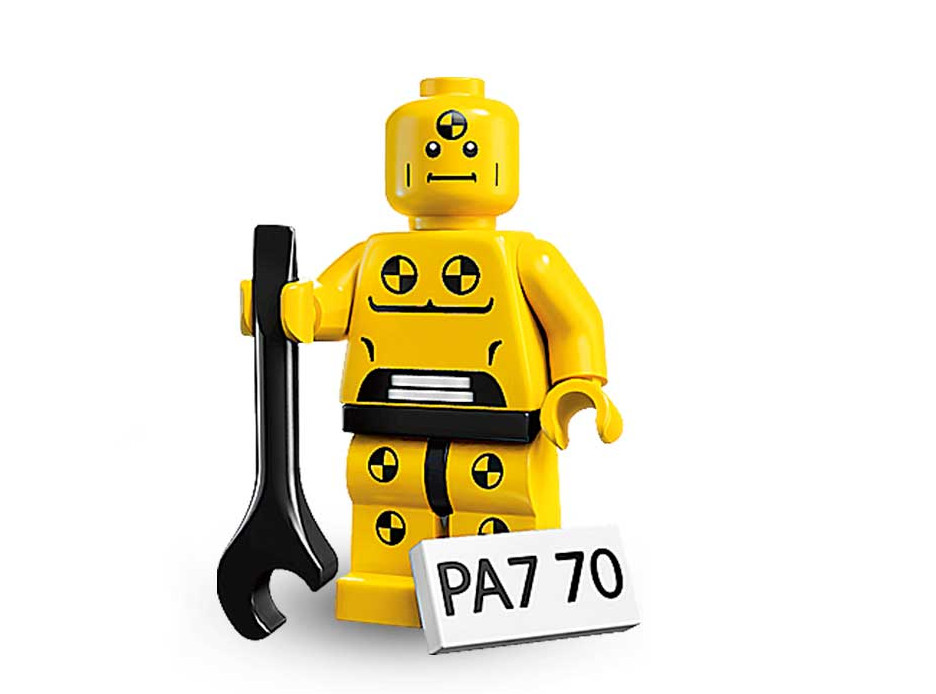
\includegraphics[width=3in]{dummy}
\caption{Block diagram of the \twi test setup.}
\label{i2c_setup}
\end{figure}
\begin{figure*}[!t]
\centering
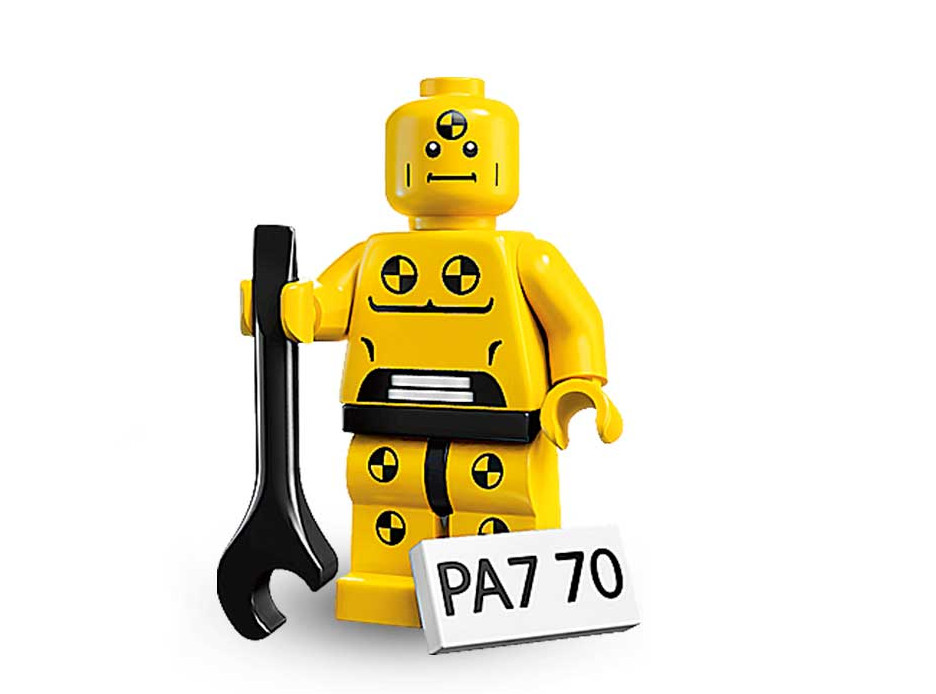
\includegraphics[width=\linewidth]{dummy}
\caption{An \twi read access measured with an oscilloscope. The upper curve represents the \scl line, the lower curve shows the \sda line.}
\label{i2c_transfer_measured}
\end{figure*}
As a practical example, an \twi transaction was measured with an oscilloscope. For this, a test board with a temperature sensor was attached to a raspberry pi running a fresh install of the Raspbian Linux distribution. On this board, a bus multiplexer is attached between the raspberry pi and the sensor. See figure~\ref{i2c_setup} for a connection scheme.
To use the \twi bus, the appropriate kernel modules (\texttt{i2c-bcm2708} and \texttt{i2c-dev}) need to be started and the package \texttt{i2c-tools} needs to be installed. Then, the following session was started, and the last transfer was recorded with an oscilloscope.

\begin{minted}[fontsize=\small]{bash}
# Tell the multiplexer to connect the
# correct bus to the pi.
pi@raspberrypi ~ $ i2cset 1 73 3 64
WARNING! This program can confuse your
I2C bus, cause data loss and worse!
I will write to device file
/dev/i2c-1, chip address 0x49, data
address 0x03, data 0x40, mode byte.
Continue? [Y/n] y
# Read the temperature sensor.
pi@raspberrypi ~ $ i2cget -y 1 76 0
0x1b
# A thumb was placed on the sensor
# to warm it up a little
pi2@raspberrypi ~ $ i2cget -y 1 76 0
0x1d
\end{minted}

Figure~\ref{i2c_transfer_measured} shows the merged screenshots from the oscilloscope, annotated with the bus actions. The read transfer is broken down into two consecutive parts: First, the master writes the address it wants to read to the slave, which will then, after a repeated start and a read command, write the desired data on the bus.




\section{Comparison of SPI and \twi}
Please refer to figure~\ref{i2c_spi_comparison_spider} for an illustration of the comparison.
To compare things, categories of comparison are needed. There are the six categories considered in this comparison:

\paragraph*{Speed}
When it comes to speed, SPI is a clear winner with some devices communicating at up to 60 Mbit/s.% and practically no overhead as handshaking is done by the \ss line.

\paragraph*{Simplicity of use}
To communicate with a device attached to the \twi bus, only it's address is needed. For SPI, the maximum clock speed, polarity and phase of the clock signal need to be known.
So, in this category, \twi is a winner.

\paragraph*{Simplicity at chip-level}
%How complicated it will be to implement a device communicating via this bus.
\twi requires a comparatively complex logic setup for bus arbitration and clock stretching. On the other hand, to implement an SPI-device, not much more than a shift register is needed.

\paragraph*{Simplicity at Board Level}
\twi and SPI will not need much space on a PCB, with \twi using 2 wires and 2 resistors and SPI using 3 lines and one more for each slave. The difference is marginal, but \twi wins in this category.

\paragraph*{Versatility}
Both SPI and \twi are used in a great number of applications. \twi allows easier attachment of components to the bus, while SPI is easier to comprehend and debug. Depending on the point of view, both buses could win, so this is a draw.

\paragraph*{Robustness}
Neither of the bus systems implement error checking or correction at protocol level. Further, with \twi, the signal lines are only driven by a relatively weak pull-up resistor during the high phase, making them more susceptible to noise, while signal lines are always actively driven with SPI.


As demonstrated, both bus systems have strengths and weaknesses. There can be no definite answer telling which bus is better as both buses were designed for different requirements. SPI is mostly used to transfer data to and from peripheral devices, \twi is prevalently used for more configuration centric communication. Systems, which can tolerate the lower communication speeds profit by the slightly smaller complexity of \twi, whereas systems requiring a higher data throughput or which rely on a guaranteed maximum time until a message has been sent, will probably prefer SPI.

%While both are at the low-speed, low-complexity range of bus systems, each has it's own unique strengths and weaknesses. SPI is mostly used to transfer data to and from peripheral devices, \twi is prevalently used for more configuration centric communication.

\begin{figure}[!t]
	\centering
	\resizebox{3in}{!}{%
		\begin{tikzpicture}
			\tkzKiviatDiagram{Speed, Simplicity of use, Simplicity at Chip, Simplicity at Board, Versatility, Robustness}
			\tkzKiviatLine[color= gray, fill= gray!20, opacity=.5](1,9.5,5,9.5,8, 6)
			\tkzKiviatLine[thick, color= black=.5](5,8,9,8,7, 7)
		\end{tikzpicture}
	}
	\caption{Comparison of the buses. Filled: \twi, Thick line: SPI.}
	\label{i2c_spi_comparison_spider}
\end{figure}



		\medskip
\section{Conclusion}
Both \twi and SPI are very mature, while still up-to-date bus systems for low-speed, low-complexity interconnection of integrated circuits.
With their wide acceptance and when used as intended, both \twi and SPI are recommendable and reliable bus systems.


\bigskip
%\vfill

\begin{thebibliography}{1}

	\bibitem{spi_mc68hc11a8}
		Datasheet of the Motorola MC68HC11A8 microcontroller describing the SPI bus.\\
		Last downloaded 2014-01-10\\
		\url{http://cache.freescale.com/files/microcontrollers/doc/data_sheet/MC68HC11A8.pdf}
		\medskip

	\bibitem{spi_c68hcp11a1vp}
		Datasheet of the Motorola MC68HCP11A1VP microcontroller\\
		Last downloaded 2014-01-10\\
		\url{http://pdf.datasheetcatalog.com/datasheet/motorola/MC68HCP11A1VP.pdf}
		\medskip

	\bibitem{spi_blockguide}
		SPI Block Guide V03.06\\
		Last downloaded 2014-01-10\\
		\url{http://www.ee.nmt.edu/~teare/ee308l/datasheets/S12SPIV3.pdf}
		\medskip

	\bibitem{microwire}
		Datasheet detailing Microwire\\
		Last downloaded 2014-01-11\\
		\url{http://www.ti.com/lit/an/snoa743/snoa743.pdf}
		\medskip

	\bibitem{i2c_standard_v2.1}
		Phillips Semiconductors: The \twi-Bus Specification, 2000\\
		Last downloaded 2014-01-10\\
		\url{http://www.cs.unc.edu/Research/stc/FAQs/Interfaces/I2C-BusSpec-V2.1.pdf}
		\medskip

	\bibitem{i2c_standard}
		NXP Semiconductors: UM10204 I2C-bus specification and user manual\\
		Last downloaded 2014-01-10\\
		\url{http://www.nxp.com/documents/user_manual/UM10204.pdf}
		\medskip

	\bibitem{pmbus}
		Homepage for PMBus, detailing it's connection to \twi\\
		Last visited 2014-01-11\\
		\url{http://pmbus.org/about/pmbusancestry}
		\medskip

	\bibitem{smbus}
		Specification of SMBus\\
		Last downloaded 2014-01-11\\
		\url{http://smbus.org/specs/smbus20.pdf}
		\medskip

	\bibitem{twi1}
		Homepage about \twi detailing TWI\\
		Last visited 2014-01-11\\
		\url{http://www.i2c-bus.org/twi-bus}
		\medskip

	\bibitem{twi2}
		Example of a datasheet using the term ``Two Wire Interface" instead of \twi\\
		Last downloaded 2014-01-11\\
		\url{http://www.atmel.com/Images/2466S.pdf}
		%\medskip

\end{thebibliography}
\enlargethispage{-5in}
\end{document}
